\documentclass[10pt,a4paper]{extarticle}
\usepackage[latin1]{inputenc}
\usepackage{amsmath}
\usepackage{microtype}
\usepackage[none]{hyphenat}
\usepackage{verbatim}
\usepackage{amsfonts}
\usepackage{amssymb}
\usepackage{enumitem}
\renewcommand{\familydefault}{\sfdefault}
\usepackage{mathpazo}
\renewcommand{\rmdefault}{put}
\usepackage{enumitem}
\usepackage[dvipsnames,svgnames]{xcolor}
\usepackage{tkz-euclide}
\usetkzobj{all}
\usepackage{graphicx}
\usepackage{tikz} 	
\usepackage{adjustbox}
\usepackage{multicol}
\usepackage{lipsum}
\usepackage[left=0.7cm,right=1cm,top=1cm,bottom=1.5cm]{geometry}
\usepackage{cancel} \usepackage{xcolor}
\usepackage{tcolorbox}
\usetikzlibrary{decorations.pathmorphing,patterns}
\usetikzlibrary{decorations.pathreplacing,calc}
 \newcommand\coret[2][red]{\renewcommand\CancelColor{\color{#1}}\cancel{#2}}
\SetLabelAlign{Center}{\hfil\makebox[1.0em]{#1}\hfil}

%%_------= solusi


% Set this =0 to hide, =1 to show

% Set this =0 to hide, =1 to show
\newtcolorbox{mybox}[1][] { colframe = blue!10, colback = blue!3,boxsep=0pt,left=0.2em, coltitle = blue!20!black, title = \textbf{jawab}, #1, } 

%---------- kunci (jika 1 ) muncul
\def\tampilkunci{1}
\newcommand{\hide}[1]{\ifnum\tampilkunci=1
%
\begin{mybox}
 #1
\end{mybox}
%
\vspace{\baselineskip}\fi}



\newcommand*\cicled[1]{\tikz[baseline=(char.base)]{\node[white, shape=circle, fill=red!80,draw,inner sep=0.5pt](char){#1};}}

\newcommand*\kunci[1]{\ifnum\tampilkunci=1
%
\tikz[baseline=(char.base)]{\node[red, shape=circle,draw,inner sep=0.5pt,xshift=2pt](char){#1};}\stepcounter{enumii}
\fi\ifnum\tampilkunci=0
%
\hspace{3pt}#1\stepcounter{enumii}
%
\fi}

\newcommand*\silang[1]{\tikz[baseline=(char.base)]{
\draw[red,thick](-0.2,-0.20)--(0.2,0.2);
\draw[red,thick](-0.2,0.20)--(0.2,-0.2);
\node[black](char){#1};
}}

\newcommand*\centang[1]{\tikz[baseline=(char.base)]{
\draw[red, very thick](-0.2,0.1)--(-0.1,0)--(0.2,0.3);
\node(char){#1};
}}

\newcommand*\merah[1]{
\textcolor{red}{#1}}
\newcommand*\pilgan[1]{
\begin{enumerate}[label=\Alph*., itemsep=0pt,topsep=0pt,leftmargin=*,align=Center] #1 
\end{enumerate}}
\newcommand*\pernyataan[1]{
\begin{enumerate}[label=(\arabic*), itemsep=0pt,topsep=0pt,leftmargin=*] #1 
\end{enumerate}}

\newcommand{\pilgani}[1]{                            \vspace{-0.3cm}\begin{multicols}{2}
 \begin{enumerate}[label=\Alph*., itemsep=0pt,topsep=0pt,leftmargin=*,align=Center]#1                     \end{enumerate}
 \phantom{ini cuma sapi, wedus, dan ayam}
 \end{multicols}}


\begin{document}


 \textbf{Pembahasan Dinamika Partikel} \phantom{ini nama siswa yang aaamengerjakan soal kuis ini }  

\begin{multicols*}{2}\raggedcolumns
\textbf{Dinamika Partikel}
\begin{enumerate}
\item $fs_{max}=\mu_s.N=0,2.mg=0.2.100=20$ N\\
pada  soal ini dikatakan bahwa ditarik ke kanan dengan gaya 12 N. Baca dicatatan bahwa jika $F<fs_{max}$ maka benda belum bergerak, sehingga $a=0$ dan gaya gesek yang bekerja akan sama dengan gaya yang menarik. \\
\textbf{Jawaban : E}

\item Untuk menentukan percepatan gunakan
\begin{align*}
\Sigma F &= \Sigma m. a\\
F\cos \theta  - f &= m.a\\
25.0,8 - \mu.N &=5.a\\
20 - 0,1 (mg - 25\sin \theta)&=5.a\\
20-0,1(50-15)&=5.a\\
a &=3.3 \text{ m/s}
\end{align*}

\item Benda saat berada pada bidang miring maka besarnya gaya berat adalah $mg\sin (\theta)$. Sedangkan gaya normalnya $mg \cos (\theta)$. maka\\
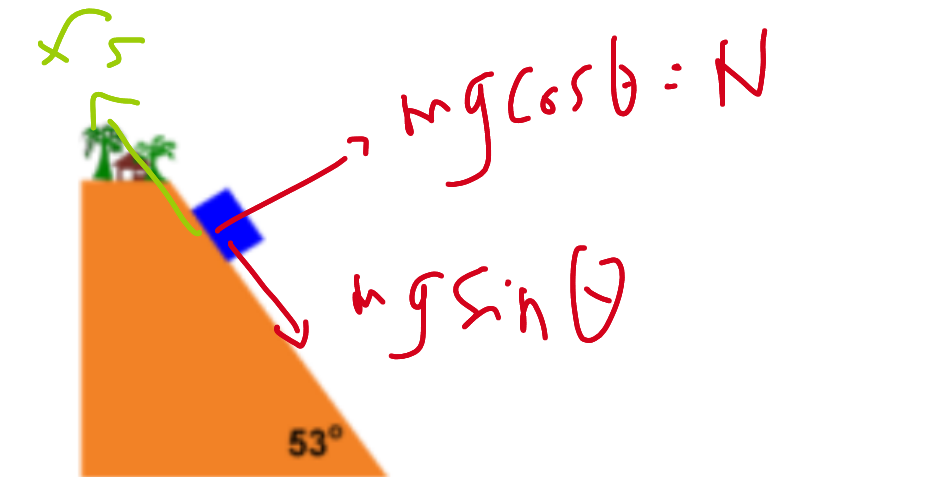
\includegraphics[width=6cm]{pic/68A3}
\begin{align*}
\Sigma F &= m.a\\
mg\sin (\theta)- f &= m.a\\
1000.0,8-\mu.mg\cos (\theta) &= m.a\\
800- 0,125 .1000.0,6&= 100.a\\
a&=7,25 \text{m/s}^2
\end{align*}
\textbf{Jawaban : D}

\item Untuk menentukan tegangan tali maka harus hitung dulu percepatannya. 


\end{enumerate}
\end{multicols*}\end{document}






